\chapter{Fundamentação Teórica}

\section{Subestações de Energia}
\label{sec:subestacao}

Atualmente, o sistema elétrico do Brasil é formado por um conjunto de usinas, subestações, linhas de transmissão e demais equipamentos, que viabilizam a produção, transmissão e distribuição de energia elétrica. A energia é gerada em usinas que variam conforme os recursos utilizados, como hidroelétricas, termoelétricas, eólicas, nucleares, entre outras, e é então transportada por linhas de transmissão até subestações de energia de empresas distribuidoras. Nestas subestações, a tensão é ajustada para os níveis adequados de consumo. Esse processo elétrico é composto por três etapas principais: geração, transmissão e distribuição (Figura \ref{fig:substation}). O sistema elétrico é composto por diversos elementos, sendo os mais destacados os geradores, responsáveis pela transformação de energia mecânica em elétrica, e os sistemas de transmissão e distribuição, que conduzem a energia até os consumidores. As subestações têm um papel fundamental ao ajustar a tensão na transmissão e distribuição, assegurando a confiabilidade e a qualidade do serviço elétrico fornecido aos clientes  \cite{lopes2012smart}.

\begin{figure}[!h]
    \centering
    \begin{minipage}{0.9\linewidth}
    \centering
    \captionsetup{justification=centering,margin=0.5cm,font=small}
    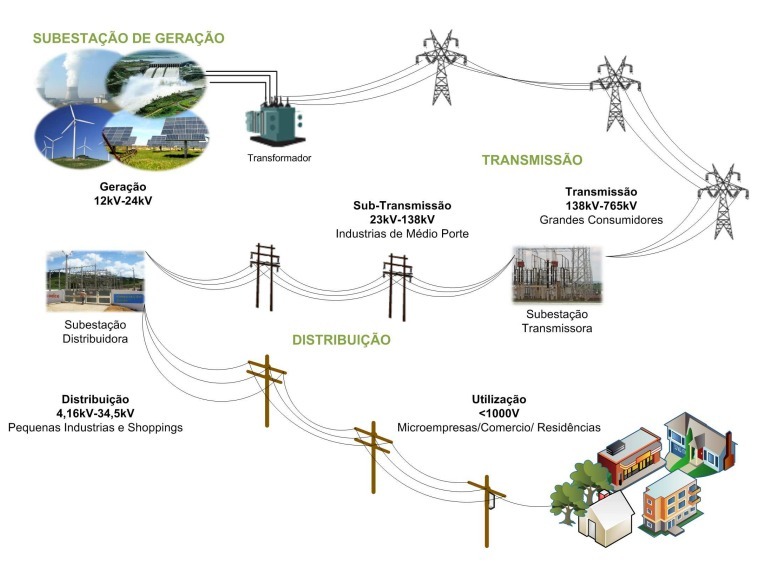
\includegraphics[width=0.9\linewidth]{img/cap2/substation.jpeg}
    \caption{Representação dos componentes do sistema de geração e transmissão de energia \cite{lopes2012smart}}.
    \label{fig:substation}
    \end{minipage}
\end{figure}

De modo geral, portanto, a energia é, obtida por geradores e transmitida para subestações primárias. Há aí a primeira aferição de qualidade dos níveis de transmissão. Após isso, a energia transformada é enviada para subestações de distribuição, alterada para níveis mais baixos para serem transmitidas para setores industriais e urbanos \cite{barreto2022proposta}.

É importante destacar que a energia produzida no Brasil é oriunda majoritariamente de fontes renováveis, em especial da geração hidroelétrica, correspondendo a 69\% de toda malha produtora. Ela é considerada uma energia limpa, de baixo custo e possui reduzida emissão de gases de efeito estufa. \cite{de2015hydroelectric}. 

Analisando mais detalhadamente as subestações, podemos afirmar que elas são encarregadas de regular a tensão tanto na transmissão quanto na distribuição de energia. Elas operam de forma autônoma, contando com sistemas supervisórios para o controle e supervisão remotos. Dentro das subestações, funções como comutação, proteção e controle também são desempenhadas. Um dos problemas que as subestações resolvem é a interrupção de curtos-circuitos, utilizando para isso disjuntores. Existem diversos tipos de subestações: as de transmissão, que conectam linhas de transmissão com diferentes voltagens; as de distribuição, que ligam linhas de transmissão a linhas de distribuição e regulam a tensão; e as subestações coletoras, que são utilizadas na geração de energia eólica para conectar a geração às linhas de transmissão. Portanto, as subestações são fundamentais para garantir a confiabilidade e a qualidade do fornecimento de energia  \cite{lopes2012smart}.

\begin{figure}[!h]
    \centering
    \begin{minipage}{0.7\linewidth}
    \centering
    \captionsetup{justification=centering,margin=0.5cm,font=small}
    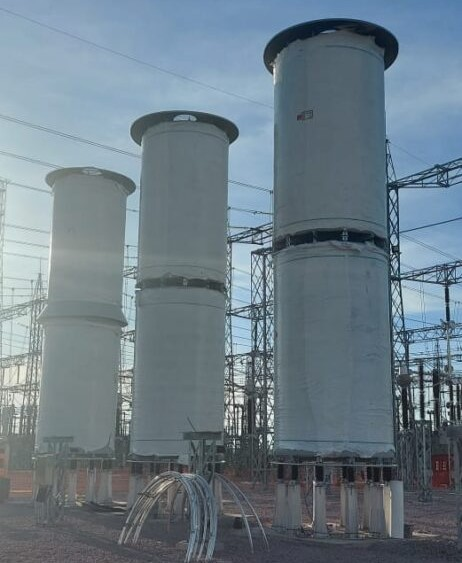
\includegraphics[width=0.7\linewidth]{img/cap2/reator-ar.jpeg}
    \caption{Reatores de Núcleo de ar em uma subestação de energia \cite{reatorNucleoDeAr}}.
    \label{fig:reator}
    \end{minipage}
\end{figure}

Dentre os diversos equipamentos que compõem a subestação de energia, um em particular será objeto de estudo neste trabalho: os reatores de núcleo de ar (Figura \ref{fig:reator}), cujo interesse reside em seu formato geométrico, que será tratado posteriormente. Nota-se que possui um corpo cilíndrico. Em seu topo, pode possuir ou não uma proteção circular contras as intempéries. Estes dispositivos são essenciais para a regulação da reatividade e controle de correntes indutivas em sistemas de transmissão e distribuição de energia. Diferentemente dos reatores de núcleo de ferro, os reatores de núcleo de ar oferecem vantagens como uma resposta mais linear e a capacidade de operar sem saturação magnética, o que os torna ideais para aplicações onde é necessário um comportamento previsível e estável \cite{de2012reatores}. 

Dentre os diversos equipamentos que compõem uma subestação de energia, este trabalho focará especificamente nos reatores de núcleo de ar. A escolha desse tipo de reator se justifica por suas características físicas quando capturadas em uma foto aérea obtida via VANT. Diferentemente de outros equipamentos presentes em seu entorno, os reatores de núcleo de ar têm um formato geométrico particular, com um corpo cilíndrico que pode incluir ou não uma proteção circular contra intempéries em seu topo. Esse formato possibilita que a RNA possa generalizar de maneira simplificada um modelo que represente o reatores, cumprindo assim a proposta do protótipo. Além disso, esses equipamentos são essenciais para distribuição de energia elétrica, atuando na regulação da reatividade e controle de correntes indutivas em sistemas de transmissão e distribuição de energia. Diferentemente dos reatores de núcleo de ferro, os reatores de núcleo de ar oferecem vantagens como uma resposta mais linear e a capacidade de operar sem saturação magnética, o que os torna ideais para aplicações onde é necessário um comportamento previsível e estável \cite{de2012reatores}.

\section{Realidade Virtual}
\label{sec:precisaorecall}

RV pode ser definida como um ambiente gerado a partir de um sistema computacional em que o usuário não apenas se sente dentro do contexto artificial, como também possibilita ao usuário a consciência de que pode navegar e interagir neste ambiente virtual. Trata-se, por isso, de uma interessante interface entre um ser humano e um computador. Nela, é possível que haja navegabilidade, interações e, principalmente, imersão em um ambiente sintético, gerado computacionalmente por meio de canais multisensoriais. Ou seja, podemos concluir que para que haja RV é necessário que existam esses três conceitos: interação, imersão e navegação \cite{kalawsky1993science}.

De acordo com \cite{cardoso2007tecnologias}, pode-se classificar a RV de duas formas diferentes: Imersiva e Não-imersiva. Na primeira, cria-se uma RV que isole o usuário do mundo real. Seus sentidos são bloqueados para recepção dos estímulos do seu entorno, para que sejam direcionados àqueles oriundos do mundo fictício. Para tanto, uma ampla variedade de equipamentos, como fones de ouvidos, luvas de dados, óculos de RV, entre outros, são empregados para os resultados esperados. Já a RV Não-Imersiva não se isola do mundo real. Ou seja, o usuário tem consciência de que está em um ambiente artificial. De modo similar, uma ampla variedade de equipamentos, convencionais e não-convencionais, é empregada para gerar essa interação, incluindo dispositivos do cotidiano, como mouses, monitores de computador.



O surgimento da RV data de 1963, em que foi apresentado uma aplicação de manipulação de objetos tridimensionais em um computador, denominada Sketchpad \cite{sutherland1963sketchpad}. A aplicação conseguia reproduzir interatividade por meio de uma caneta óptica, que era utilizada para seleção de objetos projetados em uma tela. Neste trabalho, surgiram alguns dos principais termos da RV, como representação visual, dispositivos especiais, e interações em tempo real. Em 1968, o mesmo autor do trabalho anterior, Sutherland, publicou outro trabalho marcante para a história: A Head-Mounted Three Dimensional Display \cite{sutherland1968head}. Nele, foi introduzido o conceito de imersividade para uma RV; no caso, um capacete capaz de projetar fotos diretamente aos olhos do usuário, assim como rastrear o movimento da cabeça, afim de que este movimento fosse responsivo no ambiente virtual. Seguido a isso, uma série de outros equipamentos foram desenvolvidos a fim de sofisticar as soluções do ramo e propor novos modelos. A tendência sempre prevaleceu de surgir ferramentas mais simples e acessíveis ao usuário final \cite{kirner2011evoluccao}.

Além das aplicações lúdicas, a RV atua de maneira séria e efetiva em diversas áreas técnicas. Como ferramenta para treinamento de operadores em ambientes de risco e de difícil simulação, torna-se uma alternativa viável para capacitação.  O trabalho de \cite{silva2012virtual} demonstra bem essa ideia ao investigar técnicas de RV para que uma pessoa comum, sem treinamento anterior, possa, de maneira segura à uma subestação em funcionamento e à própria pessoa e todos ao seu redor, interagir com um transformador de energia, executando todos procedimentos que teria em um ambiente real, contudo de maneira virtual. Este treinamento já seria uma base interessante para que um profissional pudesse agilizar seu treinamento no mundo real ou mesmo absorvê-los. Em trabalhos de alta periculosidade tudo é crítico; então, qualquer intervenção que possa atenuar os riscos inerentes à natureza do trabalho, traz grandes avanços ao processo de profissionalização de técnicos e pessoas interessadas. 

\section{Redes Neurais Artificiais}
\label{sec:redesneurais}

A RNA trata-se de um conjunto de técnicas que buscam simular o funcionamento do cérebro humano, a partir de algoritmos computacionais, a fim de resolver problemas específicos. Sua eficiência não necessariamente está relacionada com a quantidade de interações que as unidades de processamento que o compõem realizam entre si, uma vez que outros fatores, como tamanho do conjunto de entradas ou mesmo a qualidade delas podem influenciar o treinamento. Comparam-se as RNA à mente humana devido a sua capacidade de aprendizado, podendo generalizar funções a partir de alguns exemplos informados, e delas prever o comportamento de valores para os quais não foi fornecido a resposta esperada. A base do funcionamento da RNA está no conceito do neurônio artificial (NA), que se traduz como uma pequena unidade de processamento, capaz de receber um sinal simples, e a partir dele gerar uma resposta.  De acordo com  \cite{fleck2016redes}, a primeira noção de NA surge em 1943, no trabalho Warren McCulloch e Walter Pitts, no artigo: “A Logical Calculus of the Ideas Immanent in Nervous Activity”.

Matematicamente, o NA recebe um valor de entrada, realizando com ele o produto desse valor a um outro denominado peso. O resultado é comparado com um diferenciador: se for maior, será dada a saída verdadeira; se menor, falso. Na Figura \ref{fig:na}, esse processo é demonstrado de maneira esquemática. A operação descrita, chamada também de \textit{threshold logic}, i.e., lógica limiar, em tradução livre, mimetiza o funcionamento de um componente eletrônico chamado transistor, base do funcionamento dos processadores computacionais modernos, em que a passagem de corrente elétrica por ele é interrompida ou permitida com base no sinal de entrada \cite{mcculloch1943logical}. 

\begin{figure}[!h]
    \centering
    \begin{minipage}{1\linewidth}
    \centering
    \captionsetup{justification=centering,margin=0.5cm,font=small}
    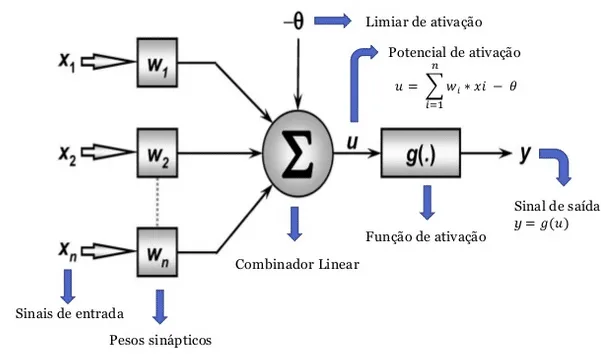
\includegraphics[width=1\linewidth]{img/cap2/na-completo.png}
    \caption{Representação de um NA \cite{adorno2017}}.
    \label{fig:na}
    \end{minipage}
\end{figure}

Aprofundando-se na álgebra relacionada do NA, pode-se visualizar o esquema do seu funcionamento na Figura \ref{fig:na}, e também acompanhar a definição de cada envolvido nesta operação \cite{deeplearningbook2023}:

\begin{itemize}
    \item \textbf{Sinais de entrada}: Constituem-se os sinais, ou valores, externos ao modelo, muitas vezes submetidos a algum tratamento prévio, responsáveis por alimentar a rede.
    \item \textbf{Pesos sinápticos}: Também chamados apenas de pesos, ponderam os sinais de cada entrada da rede.
    \item \textbf{Combinador linear}: Operação aritmética envolvendo os sinais de entrada a fim de gerar um potencial de ativação.
    \item \textbf{Bias}: O bias é um valor adicional que é somado à combinação linear das entradas antes de passar pela função de ativação, visando ajustá-la para que os dados melhor se adaptem à rede.
    \item \textbf{Limiar de ativação}: Também denominado \textit{threshold}, determina o nível adequado em que o resultado obtido pelo combinador linear pode acionar a ativação.
    \item \textbf{Potencial de ativação}: É o resultado decorrente da discrepância entre o valor gerado pelo combinador linear e o limiar de ativação. Se esse resultado for positivo, indicando \(u \geq 0\), o neurônio gera um potencial de excitação; caso contrário, o potencial será inibitório.
    \item \textbf{Função de ativação}: Sua função é restringir a saída de um neurônio dentro de um determinado intervalo de valores.
    \item \textbf{Sinal de saída}: Resultado final da saída, que pode ser utilizado como entrada para outros neurônios interligados sequencialmente.
  \end{itemize}  

  Em suma, conforme \cite{goodfellow2016deep}, a RNA, enquanto um conjunto de NA, pode ser entendido como um processador robusto, distribuído de maneira paralela, com pequenas unidades de processamento. Sua semelhança ao cérebro humano, deve-se, portanto, à capacidade de aprendizado e aos sinais sinápticos, existentes entre os neurônios, responsáveis pelo processo de armazenamento de conhecimento \cite{haykin2001redes}.
	
  De acordo com  \cite{rauber2005redes}, em 1958, após à concepção do NA, a primeira RNA a se notabilizar e a continuar sendo utilizada até o presente momento trata-se da Perceptron \cite{rosenblatt1958perceptron}. Este algoritmo possuía a capacidade de alterar os pesos dos neurônios, conforme o avanço do processamento da rede, de modo a resolver problemas da classificação linear. Seguido a ela, em 1960, houve a concepção da rede Adaline \cite{widrow1960adaptive}. Diferentemente da perceptron, esta rede já se mostrava capaz de produzir resultados que iam além dos valores binários, sendo capaz de gerar respostas de valores presentes em todo o conjunto dos números reais. O cálculo da rede Adaline era baseado na regra Delta, que era capaz de aproximar os valores dos pesos gerados para aqueles valores com menor erro possível. Ambas as redes, contudo, apresentavam uma limitação quanto à modificação dos pesos em todas suas multicamadas. Para esse cenário, foi proposto o conceito de backpropagation, ou, em tradução livre, retropropagação do erro \cite{rumelhart1986learning}. A ideia da retropropagação se inicia com o feedforward, em que todos os dados de entrada de uma RNA são transmitidos do início à camada de saída, sem nenhuma alteração de peso. Desta forma, calcula-se o erro total dessa primeira passagem, comparando o valor resultante com o esperado. Essa métrica de erro torna-se o guia para o ajuste dos pesos entre as conexões de cada neurônio. Com ela, é feito o caminho de volta, e calculado um gradiente de erro, que será o fator decisivo para a atualização dos pesos durante todo o treinamento.
  
  A topologia básica de uma rede neural é dividida em três níveis de camada: a camada de entrada, a camada oculta e a camada de saída, conforme mostrado na Figura \ref{fig:topologia}. A camada de entrada é, naturalmente, aquela que recebe os dados de entrada. Nela, cada nó representa uma característica ou atributo dos dados que estão sendo alimentados na rede neural. Por exemplo, em uma aplicação de reconhecimento de imagens, cada nó na camada de entrada pode representar um pixel da imagem. A camada oculta, que não se restringe a apenas uma, podendo ser várias, representa um processo intermediário entre a camada de entrada e a camada de saída. Cada neurônio em uma camada oculta recebe entradas das camadas anteriores, realiza algum tipo de transformação não linear dessas entradas e passa o resultado para a próxima camada. A presença de múltiplas camadas ocultas permite que a rede aprenda representações complexas e abstratas dos dados. Por fim, a camada de saída representa a camada final, e ela é responsável por gerar as saídas desejadas. A estrutura da camada de saída depende do tipo de problema que está sendo resolvido. Por exemplo, em um problema de classificação, cada nó na camada de saída pode representar uma classe diferente, e a saída pode ser interpretada como a probabilidade de pertencer a cada classe \cite{rauber2005redes}.
  
  \begin{figure}[!h]
      \centering
      \begin{minipage}{0.9\linewidth}
      \centering
      \captionsetup{justification=centering,margin=0.5cm,font=small}
      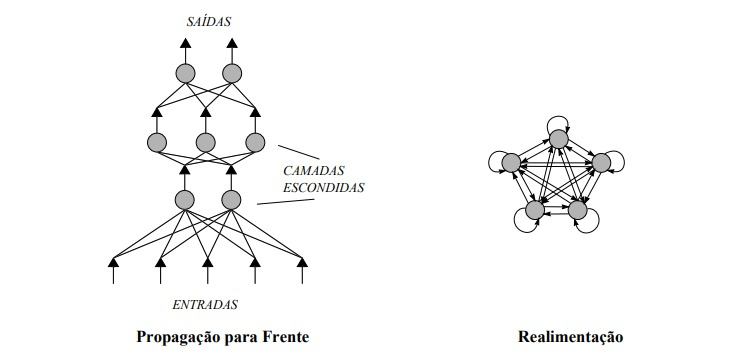
\includegraphics[width=0.7\linewidth]{img/cap2/topologia-rede.jpeg}
      \caption{Topologia básica de uma rede neural \cite{fleck2016redes}}.
      \label{fig:topologia}
      \end{minipage}
  \end{figure}  

Essencialmente, as redes neurais aprendem iterativamente ajustando os pesos de suas conexões através do processo de treinamento, onde são apresentados a um conjunto de dados de entrada e as correspondentes saídas desejadas. Com o tempo, a rede neural é capaz de aprender a mapear efetivamente os padrões nos dados de entrada para as saídas desejadas, tornando-se assim capaz de realizar tarefas como reconhecimento de padrões, classificação, regressão, entre outros \cite{haykin2001redes}.

\begin{figure}[!h]
    \center
    \begin{minipage}{0.9\linewidth}
    \center
    \captionsetup{justification=centering,margin=0.5cm,font=small}
    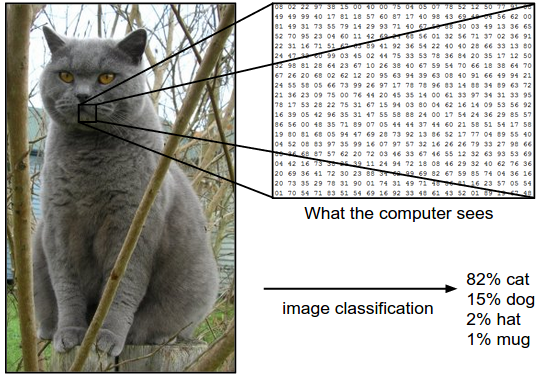
\includegraphics[width=0.7\linewidth]{img/cap2/gato.png}
    \caption{ Exemplificação de como uma imagem nada mais é que uma matriz, e como a filtragem busca padrões pré-estabelecidos dentro da imagem \cite{lima2020captcha}} 
    \label{fig:gato}
    \end{minipage}
\end{figure}

Contudo, para problemas envolvendo aprendizado por meio de imagens, a forma de lidar com as informações é diferente. De fato, imagens são dados, organizados em formato de matrizes de duas dimensões ou três dimensões (se for considerada a camada de cores), em que cada unidade de informação se chama pixel, conforme se nota no exemplo da Figura \ref{fig:gato}. Para processar esses dados, um tipo de RNA destaca-se: a Rede Neural Convolucional (RNC). Comparando ambas, nota-se que a RNA é composta por camadas intrinsecamente conectadas, em que cada neurônio de uma camada se conecta a todos os neurônios da camada seguinte. Isso faz com que ela seja adequada para dados vetorizados e para problemas de classificação e regressão sem uma estrutura espacial ou temporal específica. Por sua vez, a RNC recorre a dois tipos de camadas (Figura \ref{fig:rnc}): a convolucional, cujo objetivo é extrair características locais, e a de \textit{pooling}, responsável por manter a estrutura espacial essencial \cite{vargas2016estudo}. 

\begin{figure}[!h]
    \centering
    \begin{minipage}{0.9\linewidth}
    \centering
    \captionsetup{justification=centering,margin=0.5cm,font=small}
    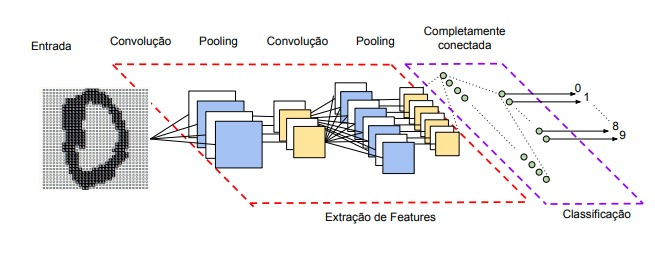
\includegraphics[width=0.7\linewidth]{img/cap2/cnn.jpeg}
    \caption{Esquema de funcionamento de uma RNC \cite{vargas2016estudo}}.
    \label{fig:rnc}
    \end{minipage}
\end{figure}

A camada de convolução, portanto, é responsável pela \textit{feature extractor}, i.e., pela extração de características de interesse em uma imagem. Basicamente, são aplicados filtros, também chamados de \textit{kernel}, à imagem a fim de buscar padrões. São comumente empregados filtros de detecção de bordas (\textit{edge detection}), desfoque (\textit{blur}), nitidez (\textit{sharpen}). Conforme na Figura \ref{fig:kernel}, cada elemento do filtro é multiplicado pelo elemento de mesma posição na região em que o filtro está sendo aplicado naquele instante. Ao final dessas operações matriciais, adiciona-se os resultados dessas multiplicações para ter um único valor como saída, que será o pixel correspondente na imagem filtrada \cite{rodrigues2023visao} . 

\begin{figure}[!h]
    \center
    \begin{minipage}{0.9\linewidth}
    \center
    \captionsetup{justification=centering,margin=0.5cm,font=small}
    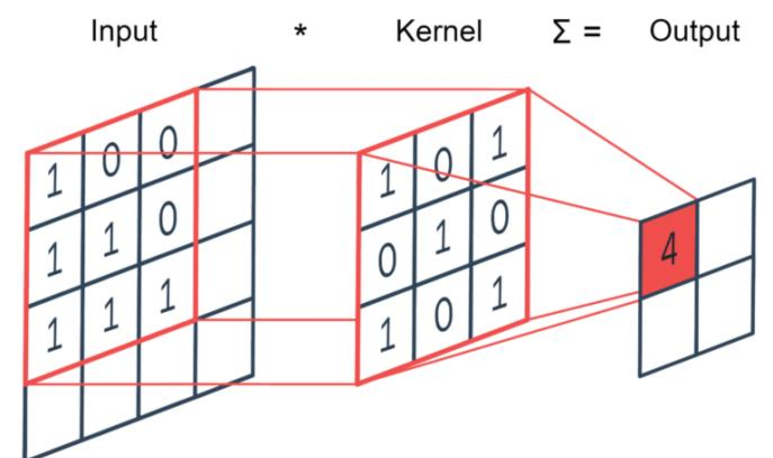
\includegraphics[width=0.7\linewidth]{img/cap2/filtro.png}
    \caption{ Operação de filtragem na camada convolucional. Nota-se que o filtro é uma multiplicação de matrizes \cite{shorthistory}} 
    \label{fig:kernel}
    \end{minipage}
\end{figure}

A camada de \textit{pooling} é aplicada após cada camada convolucional, com o objetivo de reduzir as dimensões das imagens enquanto mantém a profundidade do volume. Esse processo promove a invariância da RNC às transformações geométricas, permitindo à rede reconhecer objetos na imagem independentemente de sua posição. Além disso, o uso da camada de \textit{pooling} contribui para diminuir significativamente o custo computacional da rede. Existem diferentes tipos de \textit{pooling}, como o \textit{max pooling}, que seleciona o valor máximo em uma região específica da imagem, e o \textit{average pooling}, que calcula a média dos valores nesta região. O \textit{max pooling} é o mais comum, pois preserva as características mais salientes das imagens, enquanto reduz o ruído. A camada de \textit{pooling}, ao reduzir o tamanho espacial dos mapas de características, também ajuda a evitar um problema comum no aprendizado de máquina, em que um modelo aprende não apenas os padrões relevantes dos dados de treinamento, mas também o ruído e as particularidades específicas desses dados. Chama-se este problema de \textit{overfitting}. Evitando-o, a rede consegue construir um treinamento mais generalizável e que possa gerar resultados relevantes para dados diferentes do modelo treinado \cite{lima2020captcha}.

Por último, a camada totalmente conectada emprega uma função de ativação na sua camada de saída para realizar a classificação. Ser totalmente conectada significa que todos os neurônios da camada anterior estão ligados a todos os neurônios da camada subsequente. Ela recebe as saídas da camada de convolução e da camada de \textit{pooling} e, em seguida, utiliza essas informações para determinar a classe à qual a imagem de entrada pertence \cite{silva2018estudo}.

As RNC representam por si só uma revolução no campo da visão computacional, tornando-se a base para uma variedade de aplicações, desde reconhecimento de imagens até análise de vídeos. Entre as arquiteturas mais notáveis estão a LeNet, AlexNet, VGGNet, GoogLeNet e ResNet, cada uma contribuindo com avanços significativos em profundidade, eficiência e precisão. Além dessas, uma destaca-se em especial: a YOLO (“You Only Look Once”), uma abordagem inovadora para treinamento e detecção de objetos \cite{carboni2021sistema}.

\subsection{You Look Only Once}
\label{sec:yolo}

YOLO, uma RNC, é conhecida por sua eficácia e precisão na detecção de objetos em imagens e vídeos. Desenvolvida por Joseph Redmon, Santosh Divvala, Ross Girshick e Ali Farhadi em 2015, a arquitetura do YOLO foi apresentada em sua primeira versão no artigo "You Only Look Once: Unified, Real-Time Object Detection" \cite{redmon2016youlookonce}.

A arquitetura do YOLO é singular: ao contrário de outras RNCs que fazem múltiplas passagens pela imagem em busca de objetos, o YOLO analisa a imagem inteira de uma vez, justificando seu nome, que em tradução livre significa “você olha apenas uma vez”. Essa abordagem permite ao YOLO aplicar uma única rede neural à imagem completa. Durante o processamento, a imagem é dividida em regiões menores, e a rede prevê caixas delimitadoras, as probabilidades de existência de objetos nessas caixas, e a classe provável de cada objeto. Sua classificação, enquanto rede neural, vai além da RNC, pois ela utiliza uma arquitetura conhecida como Darknet, um tipo de rede neural profunda (variação da RNC) e sua implementação original foi desenvolvida em C, embora agora esteja disponível em várias outras linguagens de programação, graças ao apoio da comunidade e de empresas. Quando utilizada para treinamento sua estrutura básica, estabelecida em sua primeira versão, segue, evidentemente, o padrão de uma RNC. As camadas convolucionais iniciais da rede extraem características da imagem, enquanto as camadas totalmente conectadas preveem as probabilidades de saída e as coordenadas (Figura \ref{fig:rnc-yolo}). Em sua primeira versão, a rede possuia 24 camadas convolucionais seguidas por 2 camadas totalmente conectadas \cite{yoloVisaoComputacional}.

\begin{figure}[!h]
    \center
    \begin{minipage}{1\linewidth}
    \center
    \captionsetup{justification=centering,margin=0.5cm,font=small}
    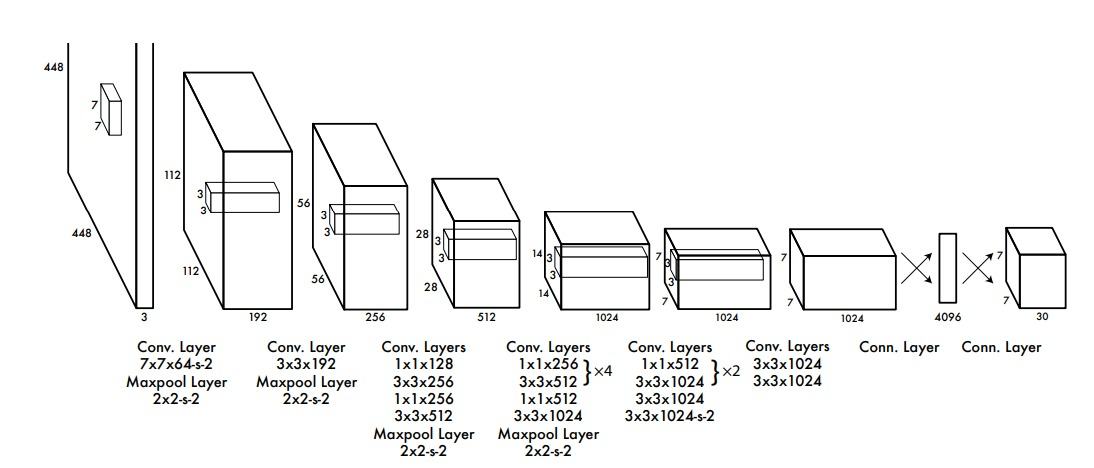
\includegraphics[width=1\linewidth]{img/cap2/RNC-YOLO.jpeg}
    \caption{ Disposição das 24 camadas convolucionais e das 2 camadas totalmente conectadas \cite{redmon2016youlookonce}} \label{fig:rnc-yolo}
    \end{minipage}
\end{figure}

Embora existam várias versões do YOLO, há um funcionamento geral da arquitetura. O primeiro passo do YOLO é dividir a imagem em uma grade de células S por S. Nas versões iniciais, essa grade era de 13x13, totalizando 169 células, enquanto nas versões mais recentes é de 19x19. Cada célula é responsável por prever/detectar 5 caixas delimitadoras, pois pode haver múltiplos objetos em uma única célula. Portanto, na versão de exemplo do YOLO, há um total de 845 caixas delimitadoras (13x13x5). Na Figura \ref{fig:yolo}, esse processo é representado. Notam-se diversas caixas, aquelas com bordas mais grossas indicam que a probabilidade de a demarcação estar representando o objeto que se propõe é alta. \cite{jiang2022review}.

\begin{figure}[!h]
    \center
    \begin{minipage}{0.9\linewidth}
    \center
    \captionsetup{justification=centering,margin=0.5cm,font=small}
    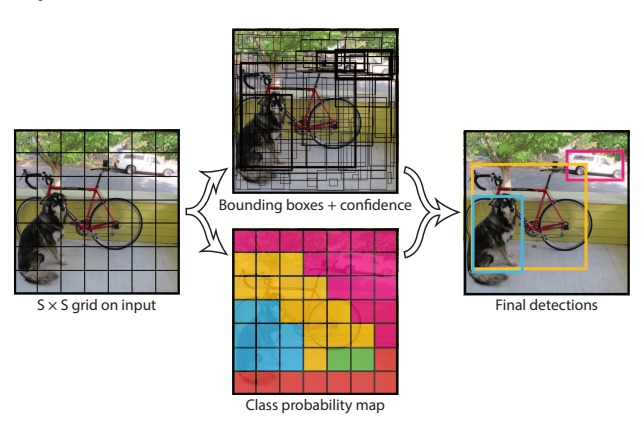
\includegraphics[width=0.7\linewidth]{img/cap2/processo-predicao-YOLO.jpeg}
    \caption{ Processo de predição da Yolo \cite{redmon2016youlookonce}} \label{fig:yolo}
    \end{minipage}
\end{figure}
A partir da YOLOv3, foram introduzidos conceitos para definir algumas partes de sua arquitetura. Primeiramente, define-se a camada de \textit{backbone}, ou espinha dorsal. Basicamente, é nesta etapa que ocorre a extração de características significativas para o processo de classificação. Ela captura características hierárquicas em diferentes escalas, com características de nível inferior (como bordas e texturas) nas camadas iniciais e características de nível superior (como partes de objetos e informações semânticas) nas camadas mais profundas. O \textit{neck}, ou pescoço, conecta a camada \textit{backbone} à \textit{head}, ou cabeça, agregando e refinando as características extraídas, muitas vezes focando em melhorar a informação espacial e semântica em diferentes escalas. A \textit{head} processa as características fornecidas pelo \textit{neck}, gerando previsões para cada candidato a objeto. Resumindo, a partir da YOLOv3, a arquitetura foi dividida em três partes: \textit{backbone} para extração de características; \textit{neck} para agregar e refinar características; e \textit{head} para fazer previsões. A espinha dorsal usa uma CNN para capturar características hierárquicas, o pescoço melhora a informação espacial e semântica, e a head gera as previsões finais, que são refinadas por pós-processamento para eliminar sobreposições \cite{terven2023comprehensive}.

Atualmente, a oitava versão da YOLO, ou, YOLOv8 , é considerada estado da arte em se tratando de análise e treinamento de imagens \cite{ultralytics2024}. YOLOv8 traz uma série de avanços significativos em relação às versões anteriores, destacando-se pela melhoria no desempenho e precisão das detecções. A arquitetura foi otimizada para equilibrar velocidade e precisão, utilizando \textit{backbones}, modernos como CSPDarknet para uma extração de características mais eficiente. O processo de treinamento foi acelerado e aprimorado com melhores métodos de regularização e otimização, enquanto a facilidade de uso e integração foi aprimorada, atendendo às demandas tanto de dispositivos de alta performance quanto de dispositivos móveis com menor capacidade de processamento \cite{hussain2023yolo}.


\subsection{Batch}
\label{sec:batch}

Um dos aspectos cruciais do funcionamento da YOLO é o conceito de \textit{batch} (em tradução livre, lote) durante o treinamento da rede neural. Ao agrupar várias imagens em lotes para processamento simultâneo, a YOLO aproveita a capacidade de processamento paralelo das GPUs, acelerando significativamente o treinamento. Durante a propagação direta, cada imagem no lote é processada pela rede neural para gerar previsões de detecção de objetos. Em seguida, a perda é calculada em relação às anotações verdadeiras, e os pesos da rede são atualizados para minimizar essa perda, usando algoritmos de otimização como o gradiente descendente. Esse processo é repetido para vários lotes de imagens até que a rede convirja para uma solução adequada. Assim, o uso eficiente de lotes na YOLO não apenas acelera o treinamento, mas também contribui para a robustez e eficácia dos modelos de detecção de objetos resultantes \cite{goodfellow2016deep}.

\subsection{Otimizadores}
\label{sec:otimizadores}

O objetivo dos algoritmos de aprendizado de máquina supervisionados é otimizar a redução de uma função objetivo, geralmente chamada de função de custo J. Reduzir essa função é crucial, pois a rede precisa aprender os pesos que melhor representam o relacionamento entre os dados, formando um modelo preditivo para fazer previsões em novos conjuntos de dados. O algoritmo de otimização mais simples para encontrar esses pesos é o Gradiente Descendente (GD), onde se realiza pequenos passos em direção ao mínimo global da função de custo. No entanto, o GD enfrenta dificuldades com conjuntos de dados muito grandes devido à sua abordagem em lote, tornando o treinamento computacionalmente caro. Uma alternativa popular é o Gradiente Descendente Estocástico (SGD, sigla para a expressão em inglês “Stochastic Gradient Descent”), que aplica atualizações de peso com base em amostras aleatórias de dados de treinamento, resultando em convergência mais rápida. O  SGD possui três parâmetros importantes que podem influenciar no treinamento da rede neural: a taxa de aprendizagem, que determina quão rápido o otimizador tentará treinar a rede neural, com uma taxa muito alta podendo levar a falhas no treinamento e uma taxa muito baixa resultando em treinamento lento; o momentum, que indica quanto a direção da mudança de peso anterior deve influenciar na etapa atual, acelerando o treinamento ao permitir que o otimizador persista em direções com histórico de melhoria; e o decay, utilizado para diminuir a taxa de aprendizagem conforme os erros diminuem durante o treinamento, evitando oscilações excessivas e permitindo uma convergência mais suave do modelo \cite{silva2018estudo}.

Além do SGD, outro algoritmo de otimização recorrente é o Adam (“Adaptive Moment Estimation”, em tradução livre, “Estimação Adaptativa de Momento”). O otimizador Adam é um algoritmo popular de otimização de gradientes utilizado em treinamento de redes neurais e outras tarefas de aprendizado de máquina. Ele calcula e mantém estimativas adaptativas dos momentos do gradiente, incluindo o primeiro momento (média) e o segundo momento (variância). Essas estimativas são utilizadas para calcular uma correção de gradiente, chamada de momento Adam, que ajusta adaptativamente a taxa de aprendizagem para cada parâmetro. Além disso, o Adam inclui termos de regularização L2 para evitar que os pesos cresçam excessivamente durante o treinamento. Essa abordagem combinada de momentos adaptativos e ajuste de taxa de aprendizagem torna o Adam eficiente, fácil de implementar e eficaz em uma variedade de problemas de otimização \cite{kingma2014adam}.

Há também uma variação do Adam, que seria o AdamW. Esta variante do otimizador Adam que inclui regularização de peso ponderada diretamente no processo de atualização dos parâmetros, ao contrário do Adam tradicional, onde a regularização é aplicada separadamente após a atualização. Isso ajuda a corrigir problemas de decaimento de pesos em modelos de aprendizado profundo, resultando em melhor desempenho e capacidade de generalização \cite{zhou2024towards}.

\subsection{Precisão e Recall}
\label{sec:precisaorecall}

A fim de avaliar o desempenho de um treinamento na arquitetura YOLO, é preciso entender os resultados fornecidos pelo modelo. De acordo com \cite{padilla2020survey}, basicamente a YOLO utiliza a métrica chamada \textit{Average Precision} (AP) (“Precisão Média”, em tradução livre). Ela se baseia no conceito de IoU (“\textit{Intersection over the Union}”, Intersecção sobre a União, em tradução livre), que calcula uma razão entre a interseção da detecção feita pelo algoritmo com relação à marcação (\textit{bounding box}) realizada em cima da área dividida pela união dessas duas áreas (Figura \ref{fig:iou}). Essa razão poderá ser comparada com um valor pré-estabelecido, o \textit{thresholds}, que será referido por L. A partir desse valor, é possível que no processo de detecção retorne três diferentes resultados na pesquisa pela classe desejada. São eles: Verdadeiro Positivo (VP), Falso Positivo (FP) e Falso Negativo (FN). VP trata-se dos resultados considerados corretos que a rede neural retorna, que seriam todos resultados que IoU > L. FP já seriam os resultados em que IoU < L, que são tidos como incorretos.FN, por sua vez, trata dos resultados totalmente fora do esperado.

\begin{equation}
    \text{Recall} = \frac{VP}{VP + FN} \tag{1}
\end{equation}
    
\begin{equation}
    \text{Precisão} = \frac{VP}{VP + FP} \tag{2}
\end{equation}

Com esses valores, pode-se calcular os resultados da saída que o treinamento da rede YOLO fornece. Em (1), tem-se o cálculo da \textit{Recall}, que calcula a capacidade da rede de detectar todos os objetos relevantes em uma imagem. Já a Precisão (2), refere-se à capacidade da rede de encontrar apenas resultados relevantes. 

\begin{figure}[!h]
    \center
    \begin{minipage}{0.6\linewidth}
    \center
    \captionsetup{justification=centering,margin=0.5cm,font=small}
    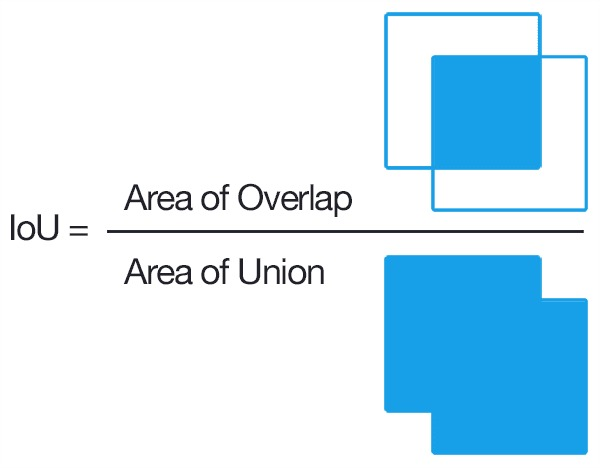
\includegraphics[width=0.7\linewidth]{img/cap2/iou.png}
    \caption{ Cálculo de IoU. \cite{padilla2020survey}}
    \label{fig:iou}
    \end{minipage}
\end{figure}

A arquitetura YOLO disponibiliza um \textit{dataset}, ou seja, um banco de imagens e \textit{weights}, comum em todas as versões, chamado de COCO (“Common Objects in Context”, que em tradução livre seria “Classes Comuns de Objetos”) com classes pré-treinadas e imagens para realização de treinamentos. A partir dele, verificou-se por meio de testes a eficiência das quatro últimas versões da YOLO, a fim de identificar se nas mais recentes houve melhoras significativas em termos de performance e precisão. Na Figura \ref{fig:precisao}, é apresentado o comparativo das versões. Nota-se que a v8, para um menor número de parâmetros que as demais, apresentou uma mAP50-95, maior que nas versões v5, v6 e v7. Além disso, com relação a velocidade de processamento, a v8 também se sobressai, com maior rapidez no processamento, ao processar maior quantidade de imagens para um mesmo intervalo de tempo \cite{padilla2020survey}.

\begin{figure}[!h]
    \center
    \begin{minipage}{0.9\linewidth}
    \center
    \captionsetup{justification=centering,margin=0.5cm,font=small}
    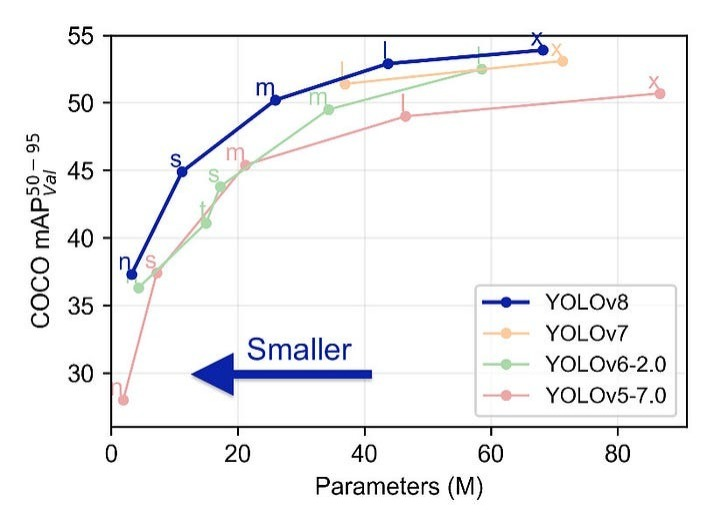
\includegraphics[width=0.7\linewidth]{img/cap2/precisao.png}
    \caption{ Aumento de desempenho da precisão média, versão 5 para 8.  \cite{ultralytics2023yolo}} 
    \label{fig:precisao}
    \end{minipage}
\end{figure}

\section{Considerações finais}

Neste capítulo, foi apresentado o arcabouço teórico necessário para o entendimento da proposta dessa dissertação. A apresentação das redes neurais, e em específico, o modo que a arquitetura da YOLOv8 sobrepõe-se em termos de eficiência em relação às demais arquiteturas abordadas em outros trabalhos científicos, demonstra o direcionamento assertivo deste trabalho. Além disso, a apresentação da RV como uma disciplina inovadora e muito útil para servir à diversos propósitos dentro da indústria e ciência, corroboram para o entendimento da proposta desta dissertação.






